\documentclass[twoside]{report}
\usepackage{iwsm}
\usepackage{graphicx}
\usepackage{amsmath, amssymb, bm}
\usepackage{booktabs}
\usepackage{lipsum}  
% Please do not specify any new definitions, any new commands,
% and do not specify any style parameters.
% The preamble of the document should be left unchanged.

\begin{document}

%***********************************************************************
% PLEASE INSERT YOUR CONTENT FROM HERE
%***********************************************************************

% Title and running title to be used as left header:
\title{Forecasting vital rates from demographic summary measures}
\titlerunning{Forecasting vital rates from summary measures}

% Authors and running list of authors to be used as right header:
\author{Carlo G.~Camarda\inst{1}}
\authorrunning{Camarda}    %% use \authorrunning{Surname 1} if only 1 author
                                    %% use \authorrunning{Surname 1 and Surname2} if two authors
                                    %% use \authorrunning{Surname 1 et al.} if more than two authors

% Institutes of all authors
% Include city and country of each institute, do not include the full address.
\institute{Institut national d'\'{e}tudes d\'emographiques (INED), Paris, France}

% E-mail of presenting author for correspondence
\email{carlo-giovanni.camarda@ined.fr}

% Brief abstract of the paper:
\abstract{In population and actuarial sciences, time-trends of summary measures (such as life expectancy or the average number of children per woman) are easy to interpret and predict. Most summary measures are nonlinear functions of the vital rates, the key variable we usually want to estimate and forecast. Furthermore smooth outcomes of future age-specific vital rates are desirable. Therefore, optimization with nonlinear constraints in a smoothing setting is necessary. We propose a methodology that combines Sequential Quadratic Programming and a $P$-spline approach, allowing to forecast age-specific vital rates when future values of demographic summary measures are provided. We provide an application of the model on Italian mortality and Spanish fertility data.}

% Keywords (at most 5):
\keywords{Vital rates forecast; Smoothing; Constrained nonlinear optimization; Summary measures.}

% Produce the title:
\maketitle

%***********************************************************************

% Sections and subsections (do not use lower levels):

\section{Introduction}
Future mortality and fertility levels can be predicted either by modelling and extrapolating rates over age and time, or by forecasting summary measures, later converted into age-specific rates. 
The latter approach takes advantage of the prior knowledge that demographers and actuaries have on possible future values of measures such as life expectancy at birth and total fertility rate. Among others, this methodology has been lately adopted by the United Nations (\v{S}ev\v{c}\'ikov\'a et al., 2016). 
In this paper, we propose a model to derive future mortality and fertility age-patterns complying with  projected summary measures. Unlike comparable approaches, we assume only smoothness of future vital rates, which is achieved by a two-dimensional $P$-spline approach as in Currie et al.~(2004), and we allow constraints to multiple series of summary measures. Since these measures are commonly nonlinear functions of the estimated penalized coefficients, Lagrangian multipliers cannot be directly implemented. We hence opted for a Sequential Quadratic Programming (SQP) procedure (Nocedal \& and Wright, 2006) to perform the associated constrained nonlinear optimization.
We illustrate our approach with two data sets. We forecast mortality of Italian females, based on future life expectancy predicted by UN World Population Prospects (2017) and a future trend of a lifespan disparity measure obtained by time-series analysis. We also forecast Spanish fertility constrained to future values of total fertility rates, mean and variance of age at childbearing, derived by time-series analysis.

\section{Model on Italian mortality data}

For ease of presentation, we formulate the model on mortality data. We suppose that we have deaths, and exposures to risk, arranged in two matrices, 
$\bm{Y} = (y_{ij})$ and $\bm{E} = (e_{ij})$, each $m \times n_{1}$, whose rows and columns are classified by age at death, $\bm{a}, \,m \times 1$, and year of death, $\bm{t}_{1}, \,n_{1} \times 1$, respectively.  
We assume that the number of deaths $y_{ij}$ at age $i$ in year $j$ is Poisson distributed with mean $\mu_{ij} \,e_{ij}$. %The value of $\mu_{ij}$ is commonly named force of mortality. 
Forecasting aims to reconstruct trends in $\mu_{ij}$ for $n_{2}$ future years, $\bm{y}_{2}, n_{2} \times 1$.

It is common practice to summarize mortality age-patterns by computing measures such as life expectancy at birth ($e_{0}$) and lifespan disparity measures. Time-trends of these summary measures are often regular and well-understood. Forecasting these time-series is therefore an easier task. Figure~\ref{fig:CamardaMort} (top-left panel) presents observed $e_{0}$ for Italian females from 1960 to 2016 along with the medium variant up to 2050 as computed by the UN. A second constraint is given by future values of $e^{\dagger}$, a lifespan disparity measure defined as the average years of life lost in a population attributable to death (Vaupel \& Canudas Romo, 2003). Future values of this measure are obtained by conventional time-series models and portrayed in the top-right panel of Figure~\ref{fig:CamardaMort}. Future mortality patterns, both by age and over time, must adhere to these predicted trends.

\begin{figure}[!ht]\centering
	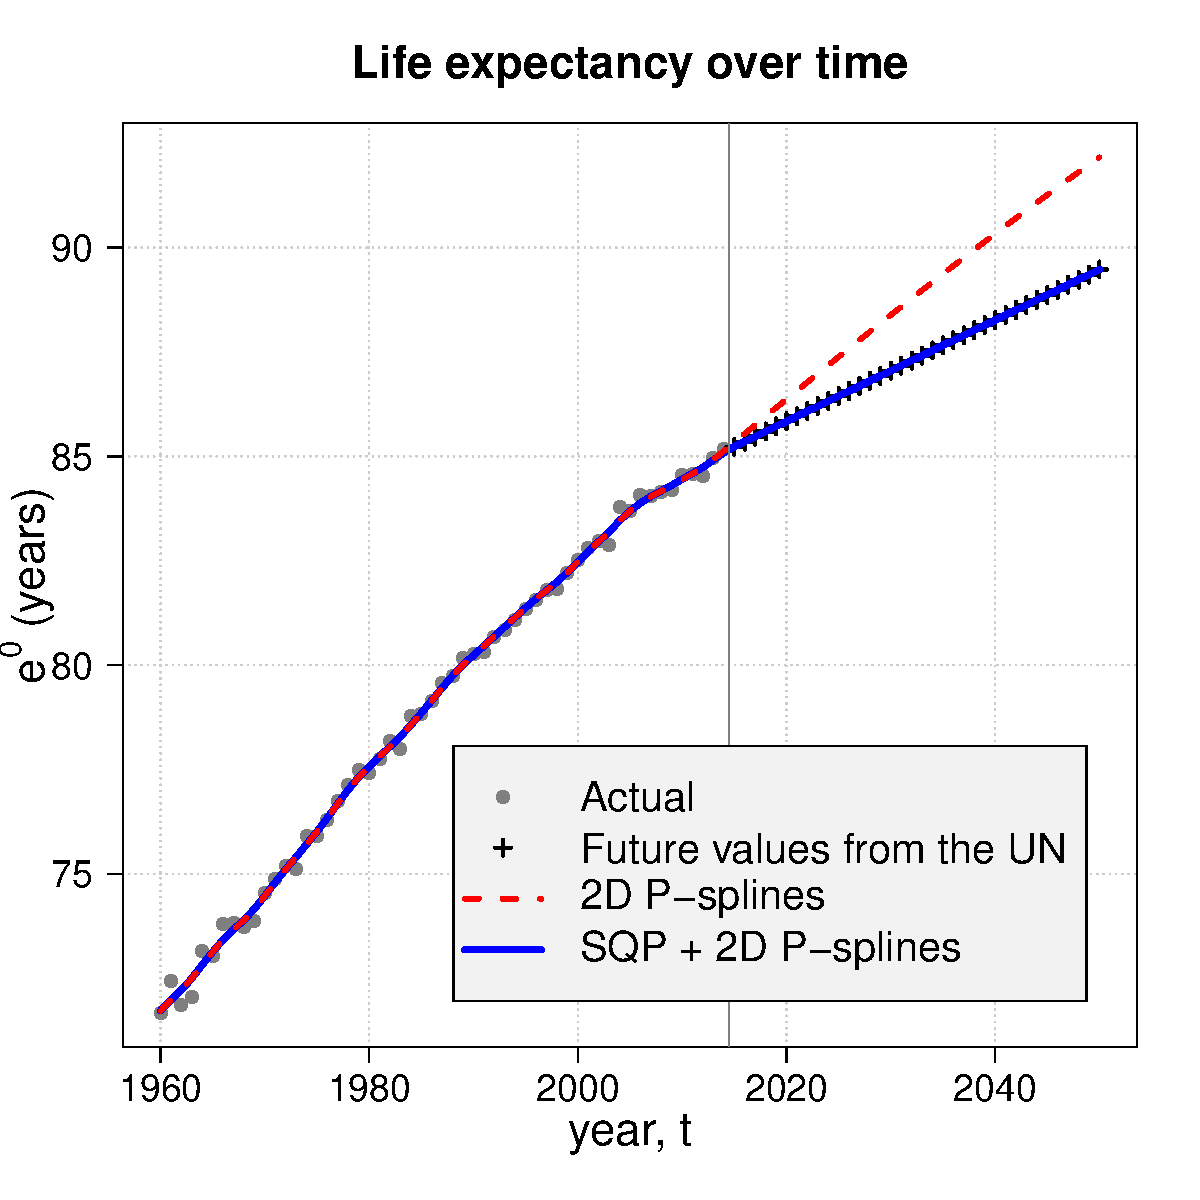
\includegraphics[scale=0.277]{Camardafig1a.pdf}
	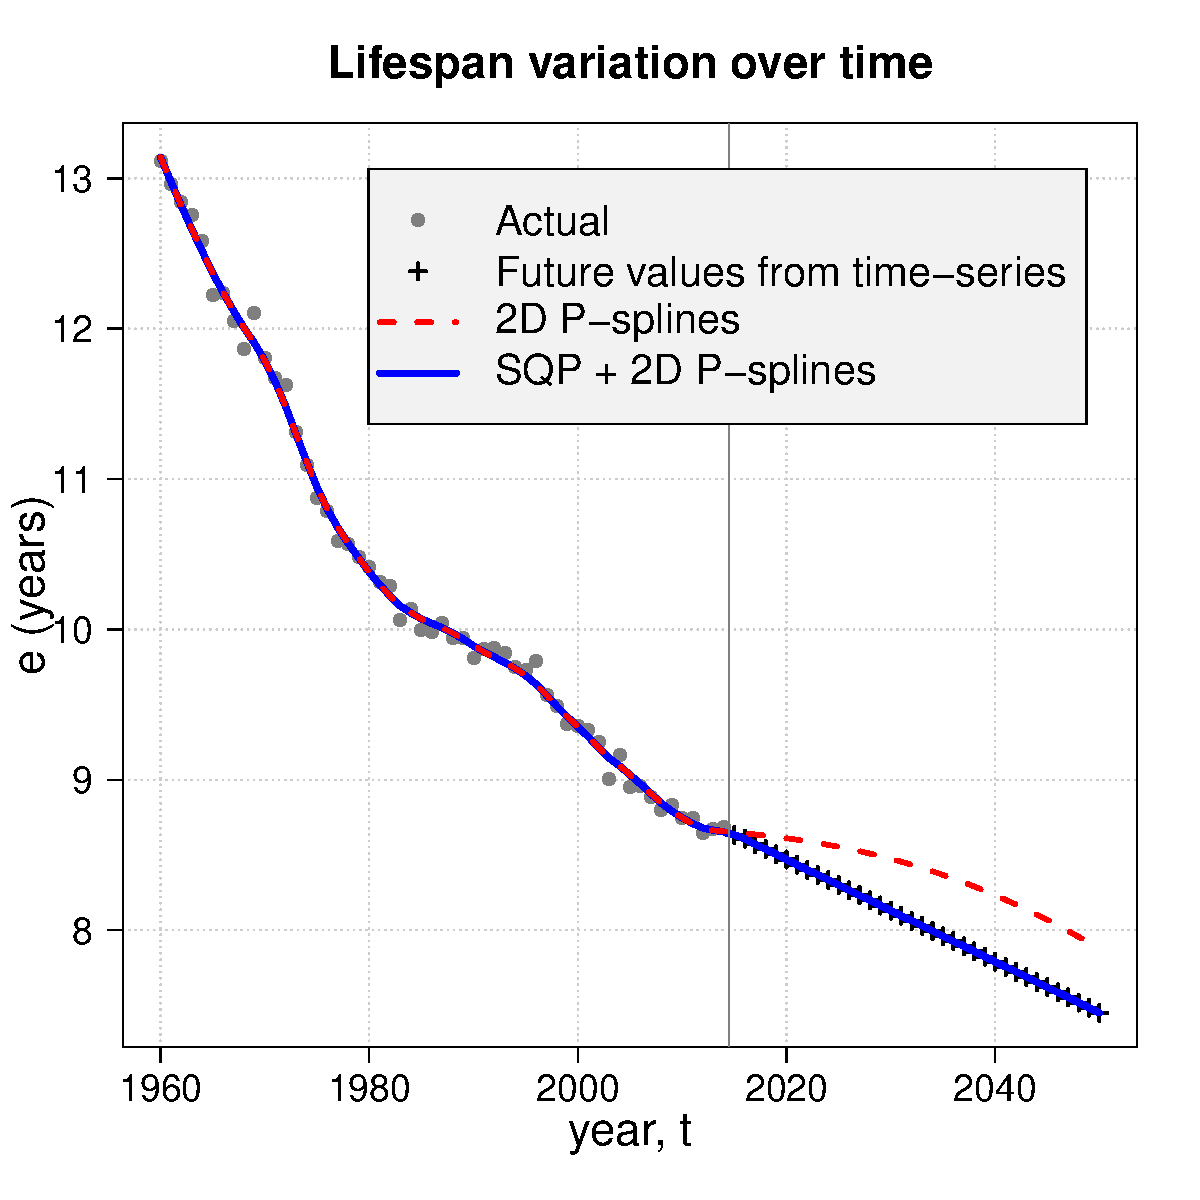
\includegraphics[scale=0.277]{Camardafig1b.pdf}
	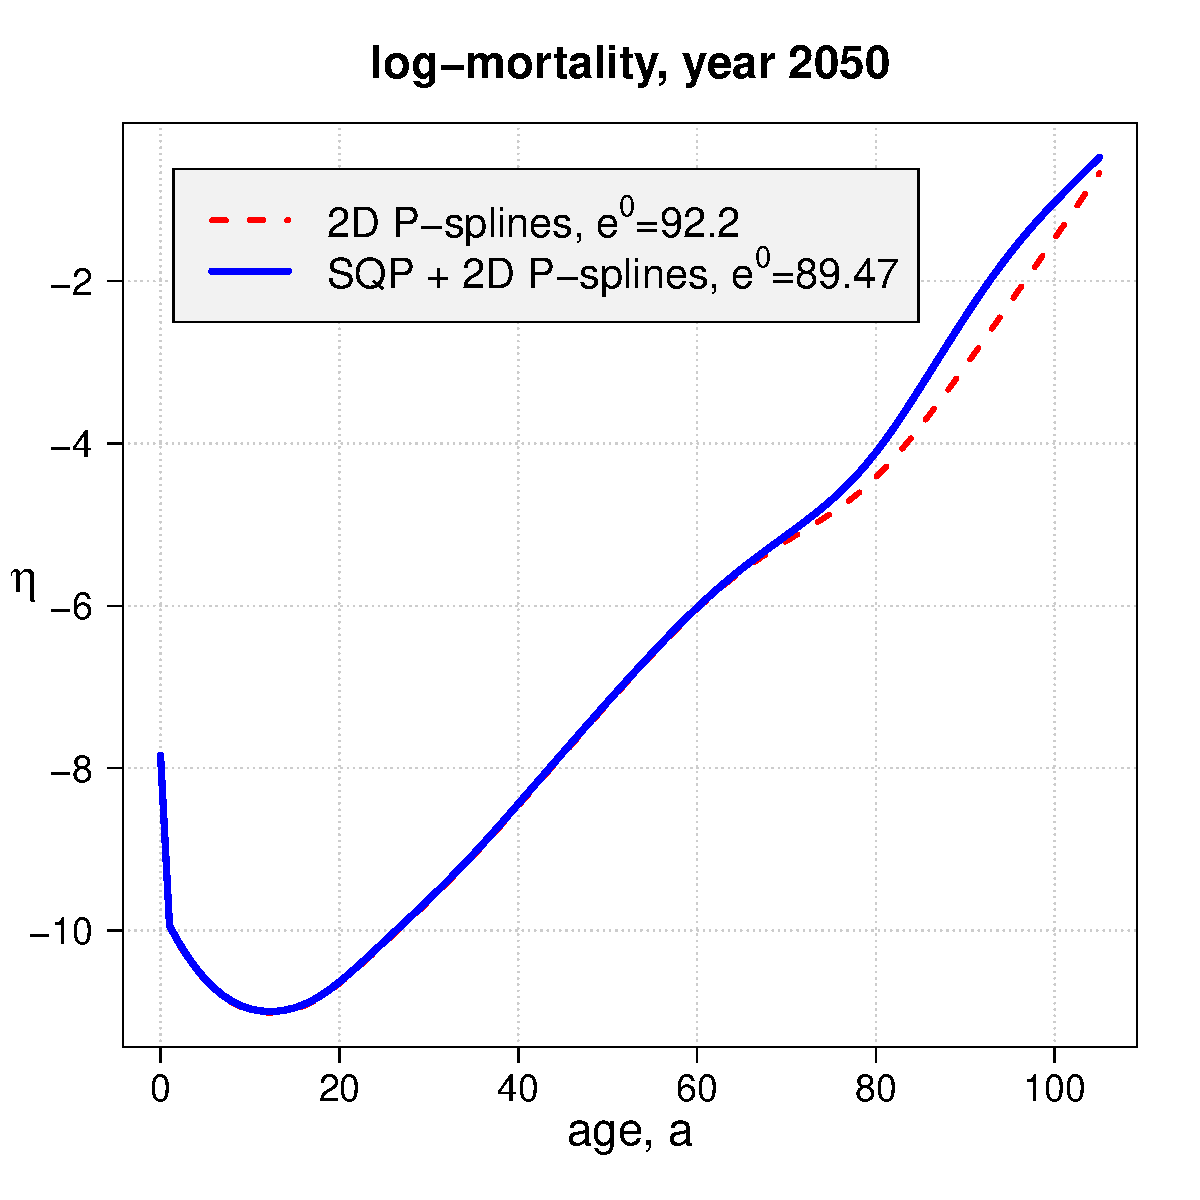
\includegraphics[scale=0.277]{Camardafig1c.pdf}
	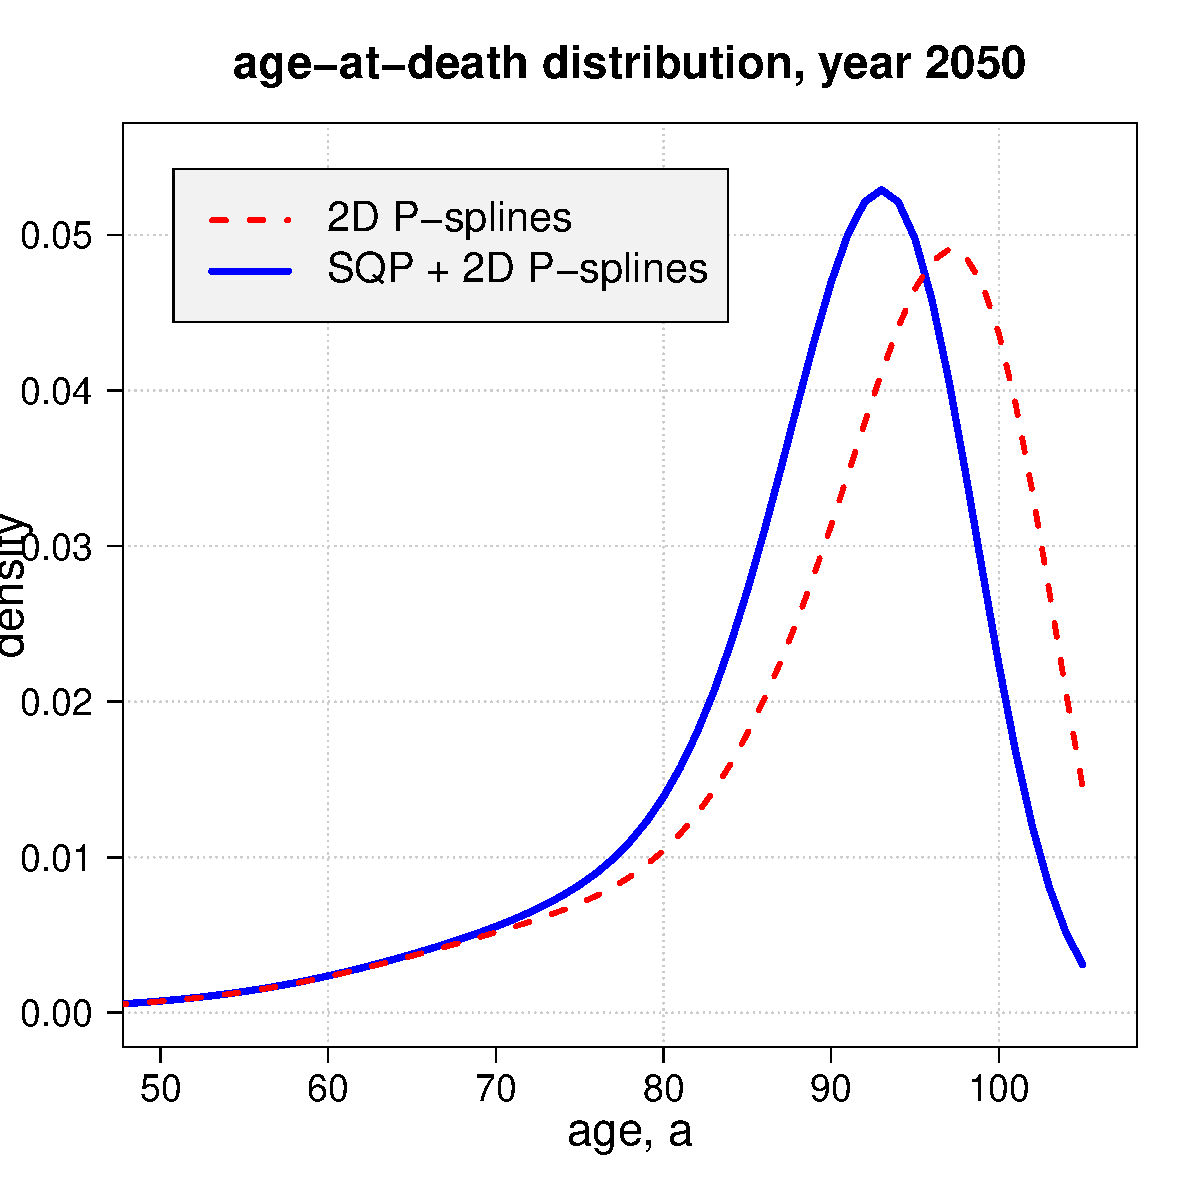
\includegraphics[scale=0.277]{Camardafig1d.pdf}
	\caption{\label{fig:CamardaMort} Top panels: Actual, estimated and forecast life expectancy at birth and lifespan disparity measure by United Nations and time-series, 2D $P$-splines and the SQP+2D $P$-splines. Bottom panels: Mortality in 2050 described by log-hazards and associated densities (ages 50+) by 2D $P$-splines and the SQP+2D $P$-splines. Italian females, ages 0-105, years 1960-2014, forecast up to 2050.}
\end{figure}

We arrange data as a column vector, that is, $\bm{y} = \verb"vec"(\bm{Y})$ and $\bm{e} = \verb"vec"(\bm{E})$ and we model our Poisson death counts as follows: $\ln(E(\bm{y})) = \ln(\bm{e})+ \bm{\eta} = \ln(\bm{e})+ \bm{B}\,\bm{\alpha}\, , $ where $\bm{B}$ is the regression matrix over the two dimensions: $\bm{B} = \bm{I}_{n_{1}} \otimes \bm{B}_{a}$, with $\bm{B}_{a} \in \mathbb{R}^{m \times k_{a}}$. Over time, we employ an identity matrix of dimension $n_{1}$ because we will incorporate a constraint for each year. Over age, $\bm{B}_{a}$ includes a specialized coefficient for dealing with mortality at age 0. In order to forecast, data and bases are augmented as follows:
\begin{equation}\label{eq:AugData}
\breve{\bm{E}} = [\bm{E} : \bm{E}_{2}]\, , \qquad 
\breve{\bm{Y}} = [\bm{Y} : \bm{Y}_{2}]\, , \qquad
\breve{\bm{B}} = \bm{I}_{n_{1}+n_{2}} \otimes \bm{B}_{a}
\, ,
\end{equation}
where $\bm{E}_{2}$ and $\bm{Y}_{2}$ are filled with arbitrary future values. If we define a weight matrix $\bm{V} = \mathrm{diag}(\verb"vec"(\bm{1}_{m\times n_{1}}:\bm{0}_{m\times n_{2}}))\,$, the coefficients vector $\bm{\alpha}$
can be estimated by a penalised version of the iteratively reweighted least squares algorithm: 
\begin{equation}\label{eq:penIRWLSfor}
(\breve{\bm{B}}^{T} \bm{V} \tilde{\bm{W}} \breve{\bm{B}} + \bm{P}) \tilde{\bm{\alpha}} =
\breve{\bm{B}}^{T}\bm{V} \tilde{\bm{W}}\tilde{\bm{z}} \, ,
\end{equation} 	
where a difference penalty $\bm{P}$ enforces smoothness behaviour of mortality both over age and time. Outcomes from this approach in terms of life expectancy and $e^{\dagger}$ are depicted with a dashed line in Figure~\ref{fig:CamardaMort} (top panels), and departures from the UN and time-series projected values are evident. 

Both life expectancy and average years of life lost are nonlinear function of the coefficients vector $\bm{\alpha}$. For a year $j$ and associated $k_{a}$ coefficients $\bm{\alpha}_{j}$, we denote mortality by $\bm{\mu}_{j} = \exp(\bm{B}_{a}\bm{\alpha}_{j})$. We can write our summary measures as follows
\begin{eqnarray}\label{eq:e0ed}
e^{0} (\bm{\alpha}_{j}) &=& \;\;\,\,\bm{1}_{m}^{\T} \, \exp[ \bm{C} \, \bm{\mu}_{j}]  + 0.5 \\
e^{\dagger} (\bm{\alpha}_{j}) &=&  - \exp[ \bm{C} \, \bm{\mu}_{j}]^{T} \, \bm{C} \bm{\mu}_{j} \nonumber
\end{eqnarray} 
where $\bm{C}$ is a $(m \times m)$ lower triangular matrix filled only with -1. 

%\begin{equation}\label{eq:Cmat}
%\bm{C} = \left[\begin{array}{rrrr}
%-1 & 0 & \cdots & 0 \\
%-1 & -1& \cdots & 0 \\
%\vdots & \vdots & \ddots & \vdots \\
%-1 & -1 & \cdots & -1
%\end{array}\right] \, .
%\end{equation}

Constrained nonlinear optimization is therefore	necessary and a SQP approach is implemented. Let denote with $\bm{N}^{0}$ and $\bm{N}^{\dagger}$ the $(k_{a}n_{2} \times n_{2})$ matrices with block-diagonal structures containing derivatives of~\eqref{eq:e0ed} with respect to $\bm{\alpha}_{j}$ for $j=n_{1}+1, \ldots n_{1}+n_{2}$:
\begin{eqnarray}\label{eq:Der}
\frac{\partial e^{0} (\bm{\alpha}_{j})}{\partial \bm{\alpha}_{j}} &=& \bm{1}_{m}^{\T} \verb"diag"[\exp(\bm{C}\bm{\mu}_{j})] \,	\bm{C} \,\verb"diag"(\bm{\mu}_{j}) \bm{B}_{a}\\
\frac{\partial e^{\dagger} (\bm{\alpha}_{j})}{\partial \bm{\alpha}_{j}} &=& - \bm{B}_{a}^{\T} \left\{ \bm{C}^{\T}[\bm{C}\bm{\mu}_{j} \circ \exp(\bm{C}\bm{\mu}_{j})] \circ \bm{\mu}_{j} \right\} + \nonumber\\
&& - \bm{B}_{a}^{\T} \left\{ [\bm{C}^{\T} \exp(\bm{C}\bm{\mu}_{j})] \circ \bm{\mu}_{j} \right\} \nonumber\, ,
\end{eqnarray}
where $\circ$ represents element-wise multiplication. Target life expectancy and lifespan disparity for future years are given by $n_{2}$-vectors $\bm{e}^{0}_{\mathrm{T}}$ and $\bm{e}^{\dagger}_{\mathrm{T}}$.

Solution of the associated system of equations at the step $\nu + 1$ is given by
\begin{equation}\label{eq:SQLalg}
\left[ \begin{array}{l}
\bm{\alpha}_{\nu+1}\\
\bm{\omega}_{\nu+1}
\end{array}\right] = 
\left[ \begin{array}{lllll}
\bm{L}_{\nu}  &:& \bm{H}^{0}_{\nu} &:& \bm{H}^{\dagger}_{\nu}\\
\bm{H}_{\nu}^{0 T}  &:& \bm{0}_{n_{2} \times n_{2}}&:&\bm{0}_{n_{2} \times n_{2}}\\
\bm{H}_{\nu}^{\dagger T} &:& \bm{0}_{n_{2} \times n_{2}} &:& \bm{0}_{n_{2} \times n_{2}}
\end{array}\right]^{-1}
\left[ \begin{array}{c}
\bm{r}_{\nu} - \bm{L}_{\nu}\bm{\alpha}_{\nu}\\
\bm{e}^{0}_{\mathrm{T}} - \bm{e}^{0} (\bm{\alpha}_{\nu})\\
\bm{e}^{\dagger}_{\mathrm{T}} - \bm{e}^{\dagger} (\bm{\alpha}_{\nu})\\
\end{array}\right] \, ,
\end{equation}
where $\bm{L}$ and $\bm{r}$ are left- and right-hand-side of the system in~\eqref{eq:penIRWLSfor}, and matrices $\bm{H}^{0} = \left[\bm{0}_{k_{a}n_{1}\times n_{2}}:\bm{N}^{0} \right]^{T}$ and $\bm{H}^{\dagger} = \left[\bm{0}_{k_{a}n_{1}\times n_{2}}:\bm{N}^{\dagger} \right]^{T}$. Vector of $\bm{\omega}$ denotes the current solution of the associated Lagrangian multipliers for both set of constraints.

Future values for $e^{0}$ and $e^{\dagger}$ forecast by the proposed method are exactly equal to the UN and time-series values (Figure~\ref{fig:CamardaMort}, top panels). The bottom panels show the forecast mortality age-pattern in 2050: the shape obtained by the suggested approach is not a simple linear function of the plain $P$-splines outcome, and differences are evident by looking at the associated age-at-death distributions. 

\section{Spanish Fertility Data}

We forecast Spanish fertility using three commonly-used summary measures: Total Fertility Rate describing average number of children per women in a given year, and mean and variance of childbearing age which measure fertility shape over age. In formulas:
\begin{eqnarray}\label{eq:FertMea}
TFR(\bm{\alpha}_{j}) &=& \bm{1}_{m}^{\T} \, \bm{\mu}_{j}\\
MAB(\bm{\alpha}_{j}) &=& \bm{\mu}_{j}^{T} \, (\bm{a}+0.5) \; / \; TFR(\bm{\alpha}_{j})\nonumber\\
VAB(\bm{\alpha}_{j}) &=& \bm{\mu}_{j}^{T} \, (\bm{a}+0.5)^2 \; / \; TFR(\bm{\alpha}_{j}) - MAB(\bm{\alpha}_{j})^2\nonumber \, .
\end{eqnarray} 

We forecast trends of these measures by time-series analysis. We then smooth and constrain future fertility age-patterns to comply forecast values of \eqref{eq:FertMea} as in \eqref{eq:SQLalg}. Summary measures as well as fertility rates in 2050 are presented in Figure~\ref{fig:CamardaFert}. Differences between proposed approach and plain 2D $P$-splines are clear. Whereas $P$-splines blindly extrapolate previous trends mainly accounting for the last observed years, the proposed approach enforces future age-patterns to adhere combinations of summary measures, guiding future fertility toward demographic meaningful trends. 

\begin{figure}[!ht]\centering
	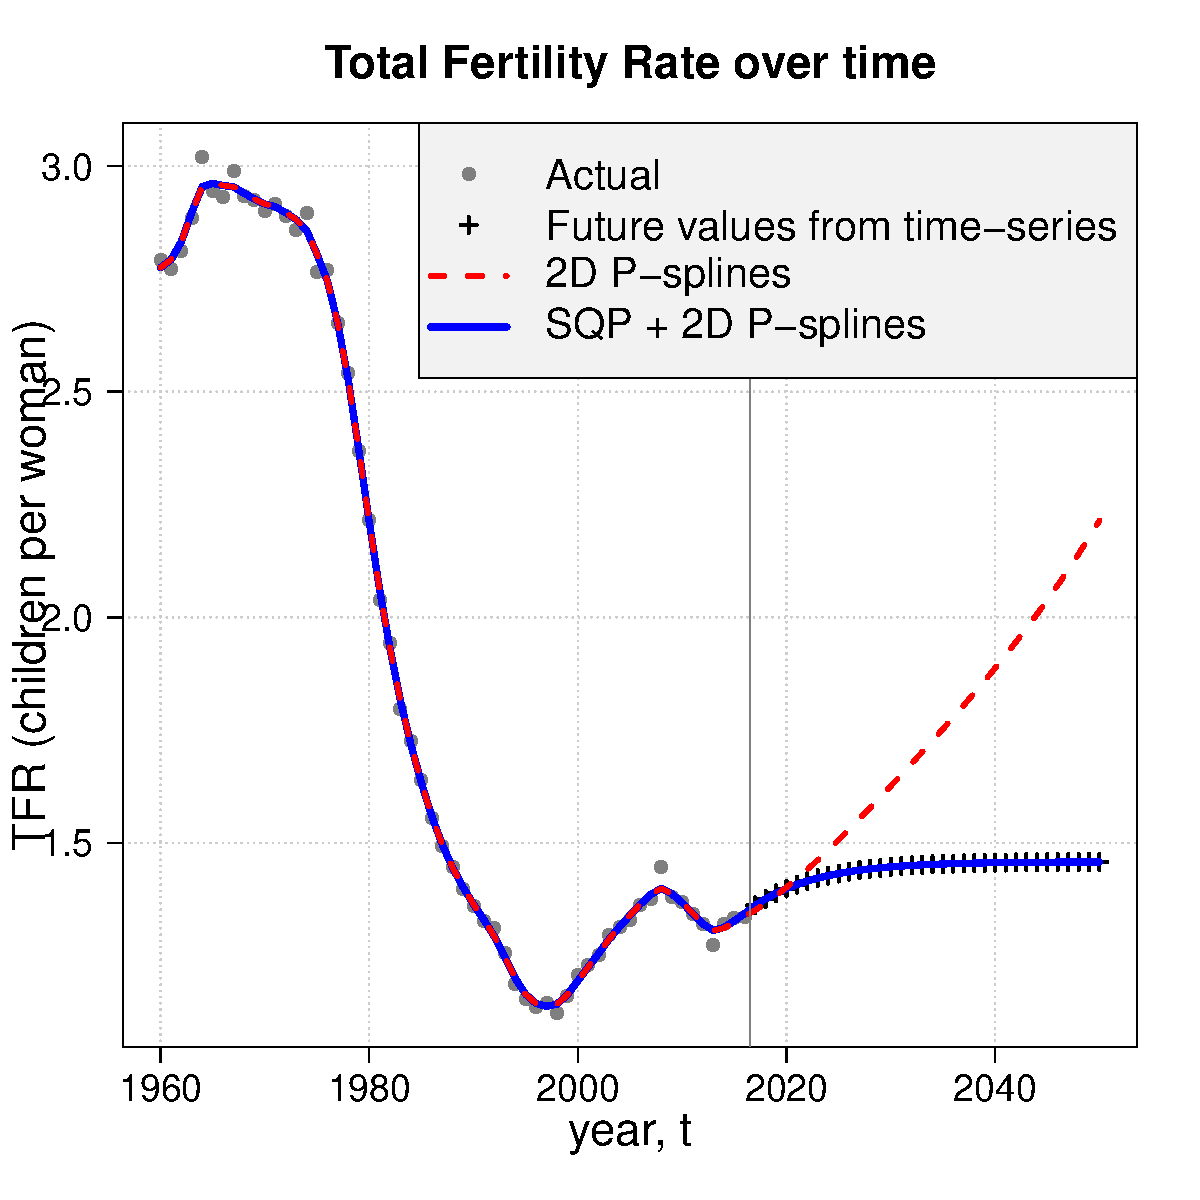
\includegraphics[scale=0.277]{Camardafig2a.pdf}
	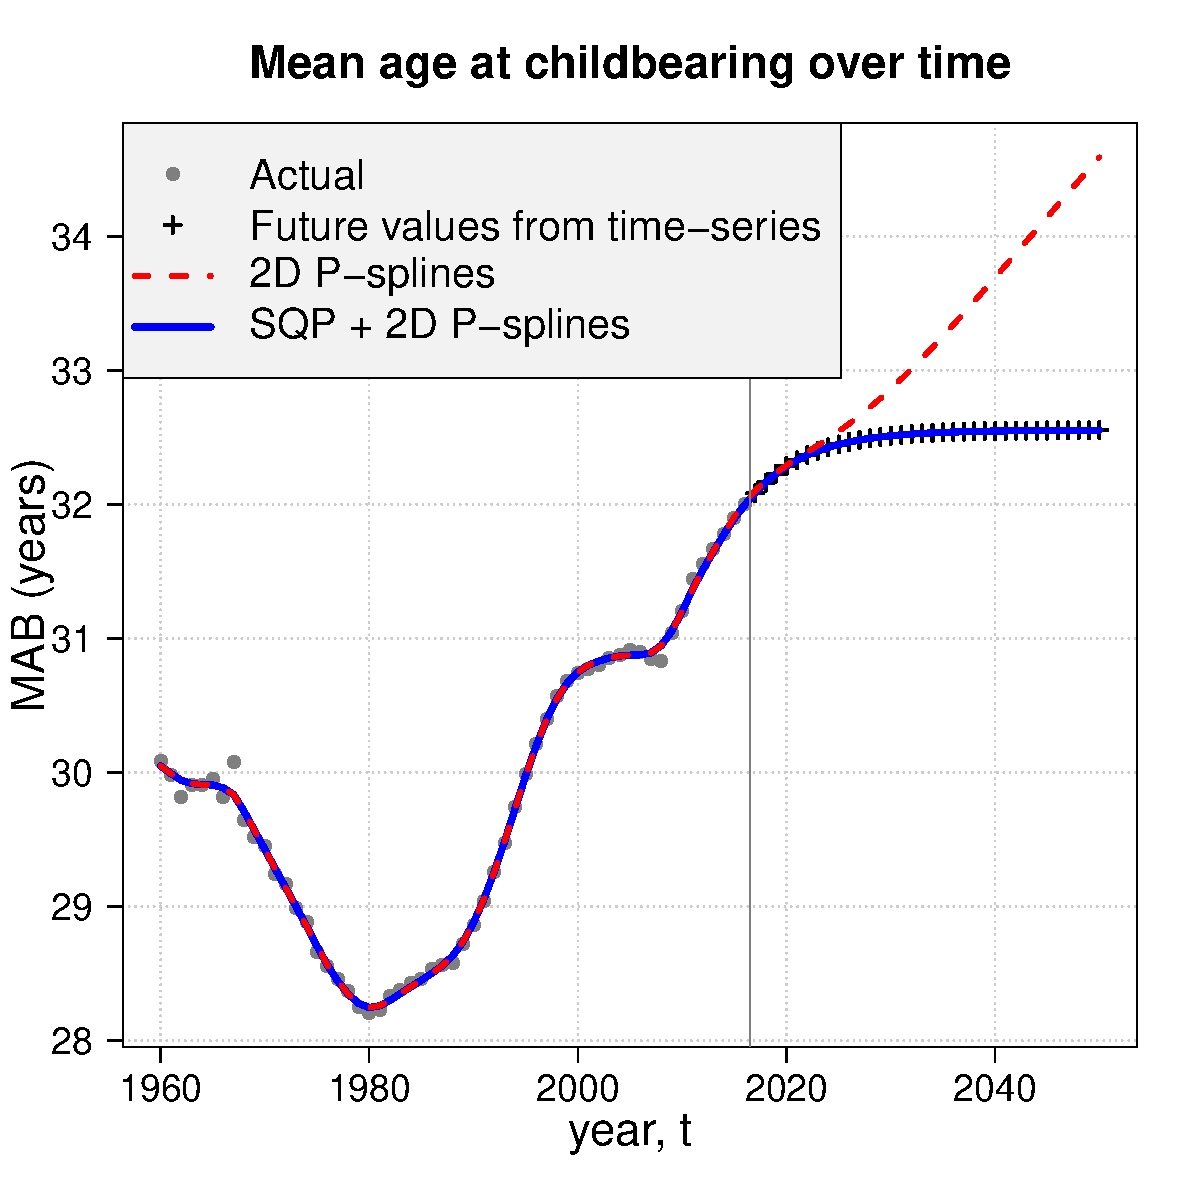
\includegraphics[scale=0.277]{Camardafig2b.pdf}
	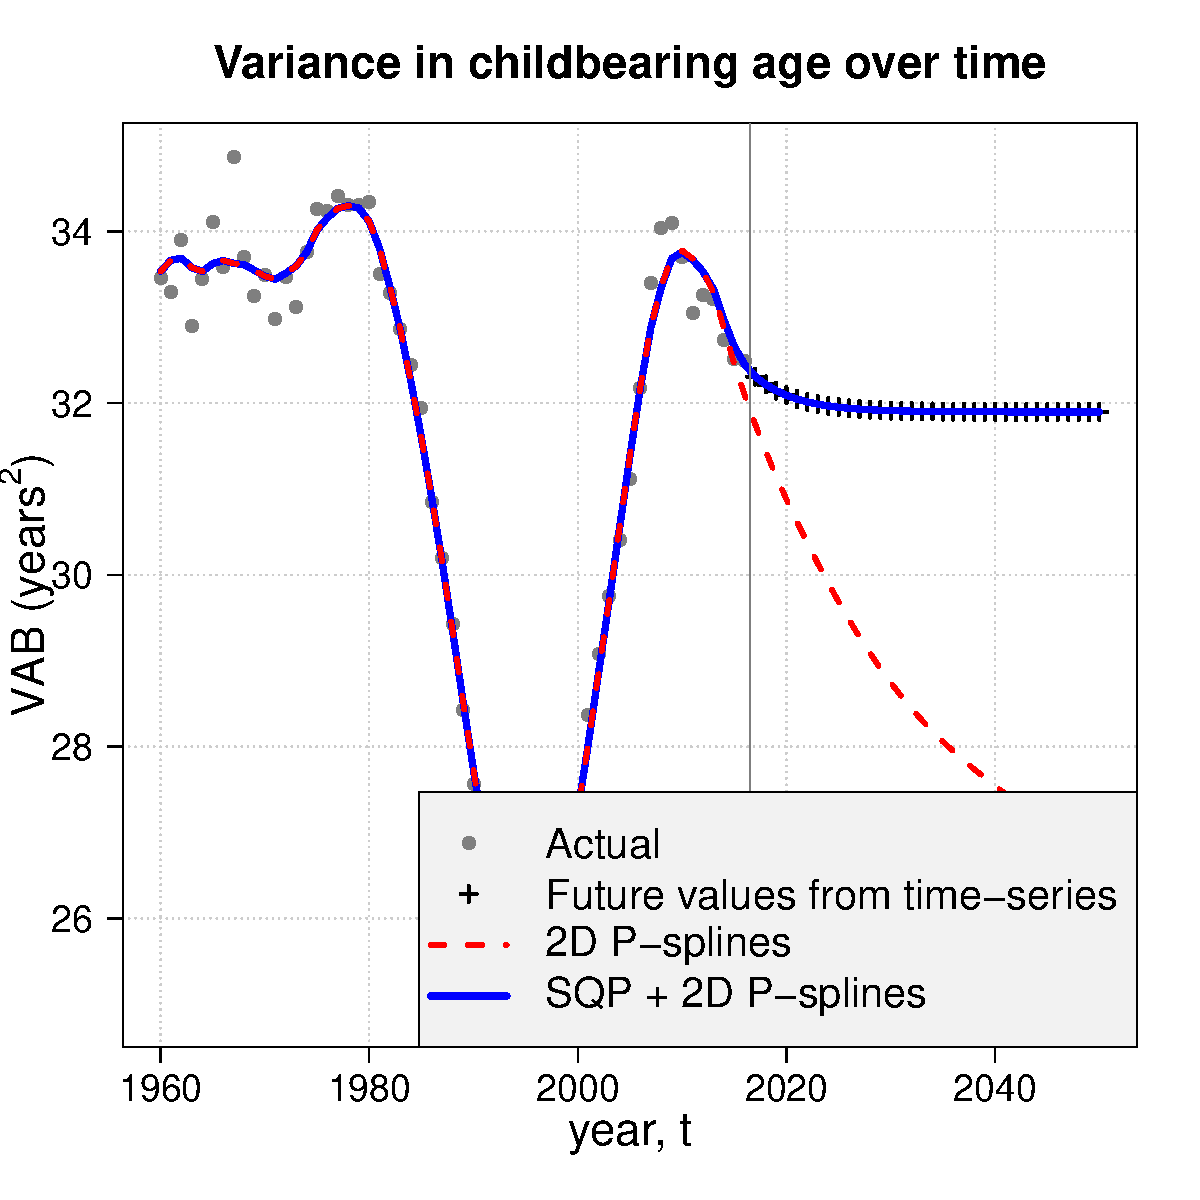
\includegraphics[scale=0.277]{Camardafig2c.pdf}
	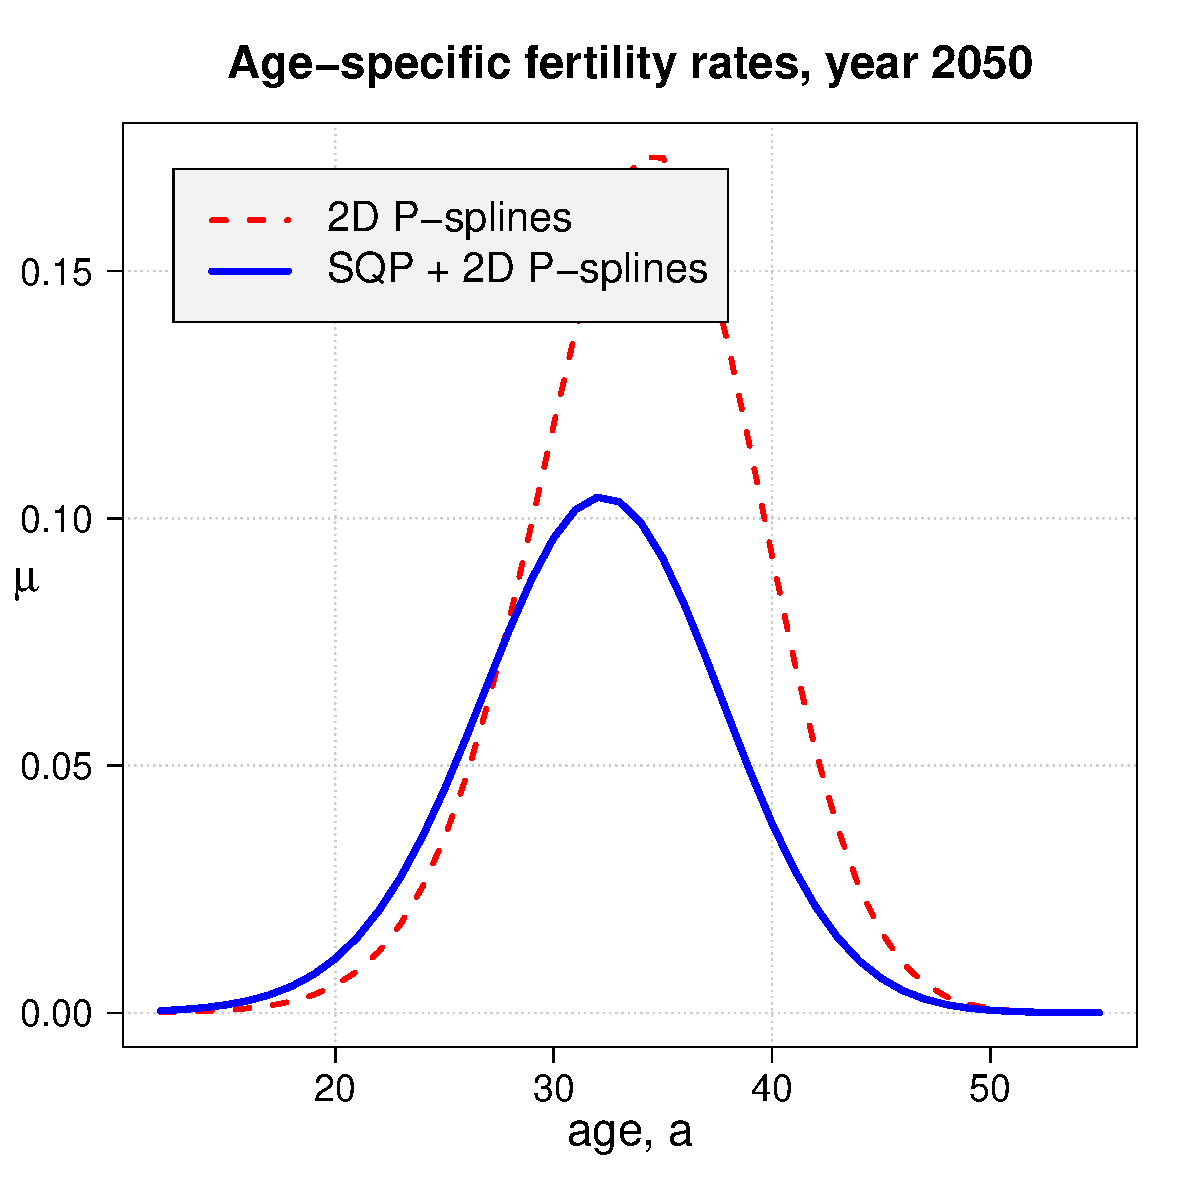
\includegraphics[scale=0.277]{Camardafig2d.pdf}
	\caption{\label{fig:CamardaFert} Top and left-bottom panels: Actual, estimated and forecast Total Fertility Rate, Mean and Variance in childbearing age by time-series analysis, 2D $P$-splines and the SQP+2D $P$-splines. Right-bottom panel: Age-specific fertility rate in 2050 by 2D $P$-splines and the SQP+2D $P$-splines. Spain, ages 12-55, years 1960-2016, forecast up to 2050.}
\end{figure}

\section{Concluding remarks}

In this paper, we combine smoothing models ($P$-splines) and optimization with nonlinear constraints (Sequential Quadratic Programming) to forecast vital rates when future values of demographic summary measures are provided. 
%The proposed approach allows to obtain smooth future mortality and fertility patterns which comply projected measures commonly easy to interpret and predict. 

We envisage further applications. Forecast of vital rates for partially completed cohorts is often relevant in population studies. For instance, final fertility history of a given cohort may be hypothesized though age-pattern is not yet observed and its estimation will be necessary. We also plan to adopt our approach to reconstruct demographic scenarios which are conventionally based on summary measures. 

From a methodological perspective, future work will be realized to incorporate uncertainty and to objectively select the amount of smoothness in future mortality and fertility age-patterns.

\references
\begin{description}
\item[Currie, I.~D. et al.]
	(2004). Smoothing and Forecasting Mortality Rates. {\it Statistical
	Modelling}, {\bf 4}, 279-298.
\item[Nocedal, J. \& Wright, S.~J.] (2006). {\it Numerical Optimization}. Springer.
\item[\v{S}ev\v{c}\'ikov\'a, H. et al.] (2016). 
Age-Specific Mortality and Fertility Rates for Probabilistic Population Projections. In R.~Schoen
(Ed.), {\it Dynamic demographic analysis}, 285\,--\,310. Springer.
\item[United Nations, Population Division] (2017). 
{\it World Population Prospects: The 2017 Revision, Volume II}. ST/ESA/SER.A/400.
\item[Vaupel \& Canudas Romo] (2003). Decomposing change in life expectancy: A bouquet of
formulas in honor of Nathan Keyfitz's 90th birthday. {\it Demography}, {\bf 40}, 201-216.
\end{description}
\end{document}

%Scenario-based projections could be also conveniently implemented using the proposed approach. 

%general model that allows to smooth and forecast future age-specific death and fertility rates complying summary measures such as life expectancy at birth and total fertility rates. 


%This study can be an elegant and convenient alternative to forecast vital rates without imposing strong structure on future mortality and fertility age-patterns. 

%Bayesian hierarchical models has been performed to obtain future life expectancy at birth and total fertility rates 
% for all countries in the world. Afterwards demographic models have been carried uut 
%mographers and actuaries have on future values of summary measures
%such as life expectancy at birth and total f

%On the one hand, vital rates are modelled using two-dimensional $P$-splines as in Currie et al.~(2004). On the other, summary measures are commonly nonlinear functions of the estimated penalized coefficients. Constrained nonlinear optimization is hence necessary and we extend a Sequential Quadratic Programming (SQP) procedure (Nocedal \& and Wright, 2006).  




%\begin{equation}\label{eq:SQLalg}
%\left[ \begin{array}{cc}
%\bm{L} & \bm{H}\\
%\bm{H}^{T} & \bm{0}_{n_{2} \times n_{2}}
%\end{array}\right]
%\left[ \begin{array}{l}
%\bm{\alpha}_{\nu+1}\\
%\bm{\omega}_{\nu+1}
%\end{array}\right] =
%\left[ \begin{array}{c}
%\bm{r} - \bm{L}\bm{\alpha}^{(\nu)}\\
%\bm{e}^{0}_{\mathrm{T}} - \bm{e}^{0} (\bm{\alpha}^{(\nu)})
%\end{array}\right] \, ,
%\end{equation}
%
%
%\begin{equation}\label{eq:SQLalg}
%\left[ \begin{array}{cl}
%\tilde{\bm{L}} & \tilde{\bm{H}}\\
%\tilde{\bm{H}}^{T} & \bm{0}_{n_{2} \times n_{2}}
%\end{array}\right]
%\left[ \begin{array}{l}
%\bm{\alpha}\\
%\bm{\omega}
%\end{array}\right] =
%\left[ \begin{array}{c}
%\tilde{\bm{r}} - \tilde{\bm{L}}\tilde{\bm{\alpha}}\\
%\bm{e}^{0}_{\mathrm{T}} - \bm{e}^{0} (\tilde{\bm{\alpha}})
%\end{array}\right] \, ,
%\end{equation}



The hat matrix is defined as
$$
H=X(X^\T X)^{-1}X^\T
$$
Please note we use \verb|^\T| to mean transposed matrices and vectors.

\subsection{Section 1.1}
Text for the first subsection within section 1. (Do you really need subsections ?)
\subsection{Section 1.2}
Text for the second subsection within section 1.
\section{Section 2}
Text for the second section. This section will have no subsections.



%***********************************************************************

% Tables can be included at any place in the text.
% As general format, use tables with horizontal lines only
% (i.e., no vertical lines separating columns).
% Start and end each table with a double horizontal line.
% Tables are incorporated using a table environment:

\begin{table}[!ht]\centering
	% A caption is put above the table and a label is defined
	% to be used for reference to this specific table.
	% Use labels which are very unlikely to be used by
	% other contributors; for example, use labels starting
	% with the surname of the first author.
	\caption{\label{smith:tab1} Caption text \textbf{ABOVE} the table.}
	% A table with three columns, where the first is left aligned,
	% the second has centred entries, and the third is right aligned,
	% is generated as follows (note: if requested, use \cmidrule{} instead of \cline{})
	\medskip
	\begin{tabular}{lcr}
		% First line:
		\toprule[0.09 em]
		% The body of the table:
		Title col1 & Title col2 & Title col3 \\
		\midrule
		row1 col1  & row1 col2  & row1 col3  \\
		row2 col1  & row2 col2  & row2 col3  \\ %
		row3 col1  & row3 col2  & row3 col3  \\
		% last line:
		\bottomrule[0.09 em]
	\end{tabular}
\end{table}

% In the text, reference to the Table can be made as follows:
We refer to Table~\ref{smith:tab1} for a summary of our main results. Have a look to Table~\ref{smith:tab2} for
an additional example.

\begin{table}[!ht]\centering
	\caption{\label{smith:tab2} Caption text \textbf{ABOVE} the table.}
	\medskip
	\begin{tabular}{lcr}
		% First line:
		\toprule[0.09 em]
		% The body of the table:
		&\multicolumn{2}{c}{Title  for cols 2 -3} \\
		\cmidrule{2-3} %
		Title1 & Title2 & Title3 \\
		\midrule
		& $a$  & $c$ \\
		& $b$  & $d$ \\ %
		\midrule[0 em]
		Total  & $a+b$  & $n$  \\
		% last line:
		\bottomrule[0.09 em]
	\end{tabular}
\end{table}



%***********************************************************************

% Figures can be included at any place in the text.
% The only allowed formats for figures are pdf files.
%
% Please, do not include figures in any other format.
%
% Use file names which are very unlikely to be used by
% other contributors; for example, use file names starting
% with the surname of the first author.
% Figures are incorporated using a figure environment:
% Make sure you specify the extension of the file (pdf)

Finally a figure (in \verb|.pdf|!)

\begin{figure}[!ht]\centering
	% You can pre-specify the width of the graph:
	\includegraphics[width=8cm]{castelo.pdf}
	% Below the figure, a caption is put, and a label is defined
	% to be used for reference to this specific figure.
	% Use labels which are very unlikely to be used by
	% other contributors; for example, use labels starting
	% with the surname of the first author.
	\caption{\label{smith:fig1} Caption text \textbf{BELOW} the figure.}
\end{figure}


% In the text, reference to the Figure can be made as follows:
We refer to Figure~\ref{smith:fig1} for a~graphical representation.


%***********************************************************************

%% Acknowledgments, if needed:
%\acknowledgments{Special Thanks to ... }

%***********************************************************************

% References should be placed in the text in author (year) form.
% The list of references should be placed below IN ALPHABETICAL ORDER.
% (Please follow the format of the examples very tightly).

%\item[Diggle, P.J., Liang, K-Y., and Zeger, S.L.] (1994).
%     {\it Analysis of Longitudinal Data}.
%     Oxford: Clarendon Press.
%\item[Green, P.J. and Silverman, B.W.] (1994).
%     {\it Nonparametric Regression and Generalized Linear Models}.
%     London: Chapman \& Hall.
%\item[Henderson, C.R.] (1973).
%     Sire evaluation and genetic trends.
%     In: {\it Proceedings of the Animal Breeding and Genetics Symposium in
%     Honour of Dr.\ L.\ Lush}, Champaign, Illinois, 10\,--\,41.
%\item[Lee, Y. and Nelder, J.A.] (1996).
%     Hierarchical generalized linear models.
%     {\it Journal of the Royal Statistical Society, Series B}, {\bf 58},
%      619\,--\,678.
%\item[Robinson, G.K.] (1991).
%     That BLUP is a good thing: the estimation of random effects (with Discussion).
%     {\it Statistical Science}, {\bf 6}, 15\,--\,51.
